\subsubsection{Iteration 2: Exploration of RL-based Control (Preliminary)}

In prior iteration, the PID method include too many parameters to adjust, causing a high-frequency control of the controller movement that human can not easy perceive. As the RL-base Control which uses DecisionRequester which can be used to control the pace easily.

\paragraph{Redesign}

I implemented a 1D control mission: regulating the drone's vertical position ($y$) within a target band $[H - R, H + R]$, where $H$ is the targetHeight and $R$ is the `acceptableRadius`.

The following two values are being observed. (1) Normalized Height Error: $\text{clip}(\frac{y - H}{R}, -k, k) / k$ (where $k$ is `errorClampK`). This maps the error to a $[-1, 1]$ range, preventing extreme spikes from destabilizing the gradient. (2) Vertical Velocity: $v_y / v_{\text{ref}}$, clipped to $[-1, 1]$.

Rewards are calculated at each decision step ($\Delta t$): (1) Event-based: A firstArrivalReward is granted upon entering the target band for the first time per episode. (2) Dense/Steady-state: A livingRewardPerSecond is granted while maintaining position within the band. (3) Shaping: A penalty proportional to the normalized excess $(|e|-R)/R$ is applied when outside the band to discourage drifting.

\paragraph{Enactment}

The agent was trained for $5 \times 10^5$ steps using the following parameters with Proximal Policy Optimization \cref{eq:ppo} approach:

\begin{itemize}
    \item Clipping parameter $\epsilon = 0.2$
    \item GAE parameters $(\lambda, \gamma) = 0.99$
    \item Neural network: a 2-layer MLP with $128$ hidden units
    \item Learning rate: $3 \times 10^{-4}$ with linear decay
\end{itemize}

To monitor progress, we implemented a color-coded feedback system, \cref{fig:train_res}: Yellow: Below target; Orange: Above target; Blue: Stable hovering.

\begin{figure}[H]
    \caption{training process}\label{fig:train_res}
    \centering
    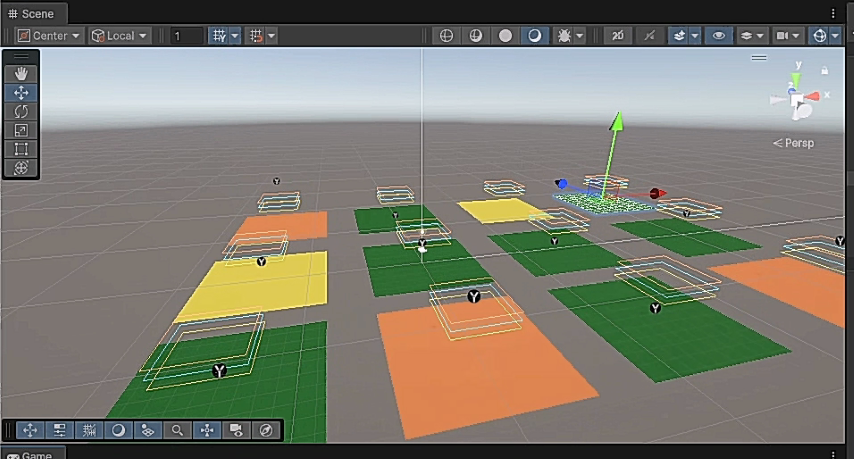
\includegraphics[width=0.8\linewidth]{img/train.png}
\end{figure}

From the train report, Cumulative Reward: Showed steady growth after 100k steps, plateauing at 400k, \cref{fig:rl_result}. Episode Length: Positively correlated with rewards; as the agent improved, it survived longer without crashing (falling too low). Environment/Cumulative Reward Histograms: also shows when training time raises, reward start to raise.

\begin{figure}[H]
    \caption{Training result of the RL agent}\label{fig:rl_result}
    \centering
    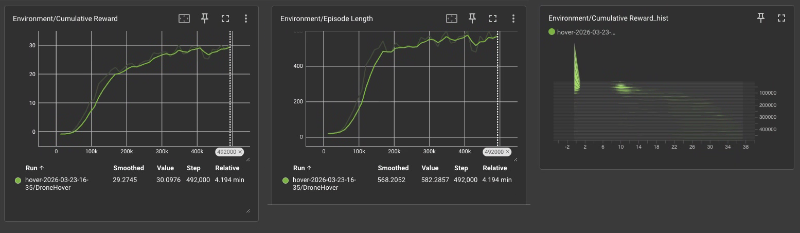
\includegraphics[width=1\linewidth]{img/result.png}
\end{figure}

The RL agent successfully learned to hover with high precision. By adjusting the DecisionRequester, we created a smoother control hint for the UI, matching the pace of human perception \cref{fig:rl_hover}.

\begin{figure}[H]
    \caption{UI prototype of the RL learning agent}\label{fig:rl_hover}
    \centering
    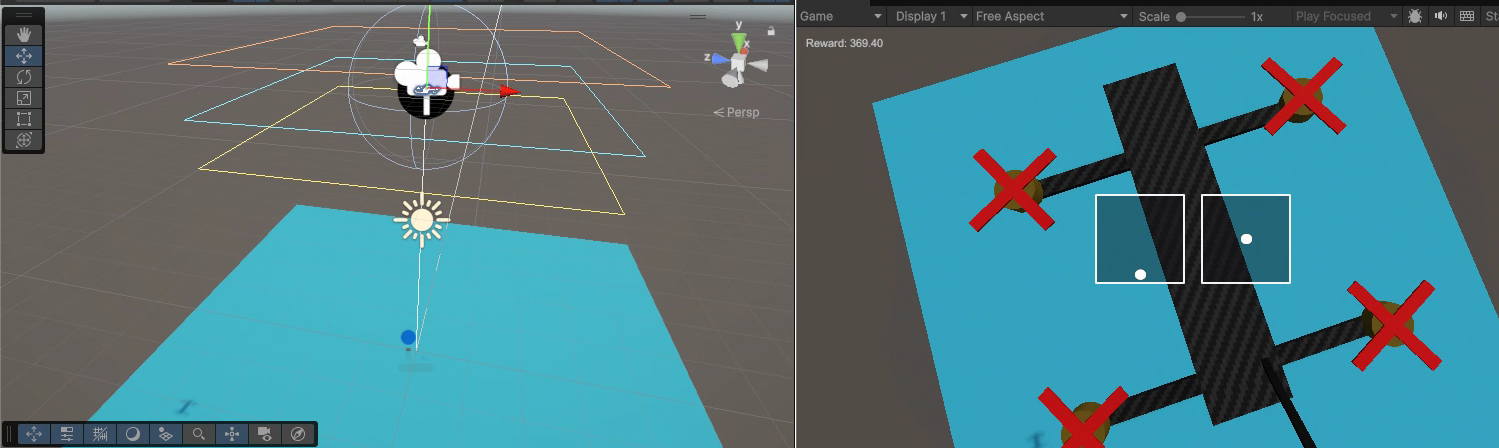
\includegraphics[width=1\linewidth]{img/hover.png}
\end{figure}

\paragraph{Analysis}

This iteration, the study focused on training a RL agent to finish hovering task. Two value were observed, a normalized height error and the vertical velocity. While if we prepare a path following task, more data should be observed. Errors in x,y,z axis, velocity in x,y,z axis and also angular velocities. Adding parameters may cause harder training as it is a black box process.

The better way should be collecting enough data and then use these data to apply a principal component approach (PCA) to find the key state variables then start the training. And this workflow can be used for a general overflow for making Reinforcement Learning based AI agent, even not target base but visual based. And this is exceeding this study, should start another to continue.